\documentclass[11pt,a4paper]{article}

\usepackage[T1]{fontenc}
\usepackage[utf8]{inputenc}
\usepackage[english]{babel}
\usepackage[a4paper,top=2.25cm,bottom=2.35cm,left=2.5cm,right=2.5cm,headsep=12pt]{geometry}
\usepackage{amsmath,amssymb,mathtools}
\usepackage{enumitem}
\usepackage{eurosym}
\usepackage{graphicx}
\usepackage{xcolor}
\usepackage{microtype}
\usepackage{avant}
\usepackage{mathptmx}
\usepackage{titlesec}
\usepackage{fancyhdr}
\usepackage{mdframed}
\usepackage{tikz}
\usepackage{needspace}
\usepackage{hyperref}
\usetikzlibrary{arrows.meta,positioning}

\definecolor{PPEBurgundy}{RGB}{112,28,47}
\definecolor{PPENavarraRed}{RGB}{211,32,46}
\definecolor{PPEGold}{RGB}{185,143,57}
\definecolor{PPEAccentLight}{RGB}{248,235,238}
\definecolor{PPEInk}{RGB}{37,31,33}
\definecolor{PPEMuted}{RGB}{101,83,88}

\hypersetup{colorlinks=true,linkcolor=PPEBurgundy,urlcolor=PPEBurgundy}
\setlength{\parindent}{0pt}
\setlength{\parskip}{0.45em}
\setlist[itemize]{topsep=0.3em,itemsep=0.2em,leftmargin=1.5em}
\setlist[enumerate]{topsep=0.35em,itemsep=0.35em,leftmargin=1.9em}
\raggedbottom
\allowdisplaybreaks[2]

\titleformat{\section}
  {\sffamily\bfseries\large\color{PPEInk}}
  {\color{PPEBurgundy}\thesection}{0.8em}{}
\titlespacing*{\section}{0pt}{1.35em}{0.5em}

\newmdenv[
  skipabove=0.7em,skipbelow=0.85em,
  leftline=true,rightline=false,topline=false,bottomline=false,
  linewidth=3pt,linecolor=PPEBurgundy,backgroundcolor=PPEAccentLight,
  innerleftmargin=0.8em,innerrightmargin=0.8em,
  innertopmargin=0.55em,innerbottommargin=0.55em
]{solutionbox}

\newmdenv[
  skipabove=0.65em,skipbelow=0.75em,
  leftline=true,rightline=false,topline=false,bottomline=false,
  linewidth=2pt,linecolor=PPEGold,backgroundcolor=white,
  innerleftmargin=0.75em,innerrightmargin=0.75em,
  innertopmargin=0.45em,innerbottommargin=0.45em
]{tipbox}

\pagestyle{fancy}
\fancyhf{}
\fancyhead[LE,LO]{\sffamily\small Microeconomics \textbar{} Final Examination \textbar{} Answer sheet}
\fancyhead[RE,RO]{\sffamily\small\color{PPEBurgundy}\thepage}
\fancyfoot[C]{\sffamily\scriptsize\color{PPEMuted}Companion to the Final Examination}
\renewcommand{\headrulewidth}{0.45pt}
\renewcommand{\headrule}{\hbox to\headwidth{\color{PPEGold}\leaders\hrule height \headrulewidth\hfill}}
\setlength{\headheight}{15pt}

\newcommand{\MRS}{\operatorname{MRS}}
\newcommand{\MRTS}{\operatorname{MRTS}}

\begin{document}

\begin{center}
  \IfFileExists{assets/branding/unav-logo-black.png}{%
    
\includegraphics[width=0.28\textwidth]{assets/branding/unav-logo-black.png}%
  }{%
    {\sffamily\bfseries\Large Universidad de Navarra}%
  }\par
  \vspace{0.5em}
  {\sffamily\color{PPENavarraRed}\large\textsc{Politics, Philosophy and Economics}\par}
  \vspace{0.3em}
  {\color{PPEGold}\rule{0.72\textwidth}{1.3pt}\par}
  \vspace{0.55em}
  {\sffamily\bfseries\color{PPEBurgundy}\LARGE Final Examination: Microeconomics\par}
  \vspace{0.16em}
  {\sffamily\large Worked answer sheet --- Full course\par}
\end{center}

\begin{solutionbox}
\textbf{Marking note.} The answer key gives one full-credit method. Award
credit for equivalent correct reasoning, notation, diagrams, and calculations.
The multiple-choice score is \(+1\) for correct, \(-0.25\) for wrong, and
\(0\) when blank.
\end{solutionbox}

\section{Multiple-choice key \hfill (33 points)}

\begin{center}
\renewcommand{\arraystretch}{1.45}
\begin{tabular}{c|ccccccccccc}
Question & 1 & 2 & 3 & 4 & 5 & 6 & 7 & 8 & 9 & 10 & 11\\ \hline
Answer   & B & C & B & B & B & B & A & B & A & B & B\\[0.25em]
Question & 12 & 13 & 14 & 15 & 16 & 17 & 18 & 19 & 20 & 21 & 22\\ \hline
Answer   & A & C & B & B & B & B & A & A & A & B & B\\[0.25em]
Question & 23 & 24 & 25 & 26 & 27 & 28 & 29 & 30 & 31 & 32 & 33\\ \hline
Answer   & A & A & B & C & B & A & A & A & A & A & A
\end{tabular}
\end{center}

\begin{tipbox}
\textbf{Coverage check.} The key assesses foundations, consumer theory,
production and cost, market structures, general equilibrium, market failures,
game theory, mechanism design, auctions, and behavioural economics.
\end{tipbox}

\section{Utility maximisation \hfill (10 points)}

\textbf{34.a Budget line.} The constraint is
\[
20x_1+10x_2=160
\qquad\Longleftrightarrow\qquad
\boxed{x_2=16-2x_1.}
\]
It has intercepts \((8,0)\) and \((0,16)\), and slope
\[
\boxed{-\frac{p_1}{p_2}=-2.}
\]

\textbf{34.b Substitution method.} Substituting \(x_2=16-2x_1\) gives
\[
u(x_1)=x_1^{1/4}(16-2x_1)^{3/4}.
\]
Because the fourth power is an increasing transformation for non-negative
utility, it is simpler to maximise
\[
v(x_1)=u(x_1)^4=x_1(16-2x_1)^3.
\]
Thus
\[
v'(x_1)
=(16-2x_1)^3-6x_1(16-2x_1)^2
=(16-2x_1)^2(16-8x_1).
\]
The interior first-order condition is
\[
16-8x_1=0
\quad\Longrightarrow\quad
x_1^*=2.
\]
The budget line then gives
\[
x_2^*=16-2(2)=12.
\]

\textbf{34.c MRS method.} The marginal utilities are
\[
MU_1=\frac14x_1^{-3/4}x_2^{3/4},
\qquad
MU_2=\frac34x_1^{1/4}x_2^{-1/4}.
\]
Hence
\[
\MRS_{1,2}=\frac{MU_1}{MU_2}
=\frac13\frac{x_2}{x_1}.
\]
At an interior optimum,
\[
\frac13\frac{x_2}{x_1}=\frac{p_1}{p_2}=2
\quad\Longrightarrow\quad
x_2=6x_1.
\]
Using the budget constraint,
\[
20x_1+10(6x_1)=160
\quad\Longrightarrow\quad
80x_1=160
\quad\Longrightarrow\quad
x_1^*=2,\qquad x_2^*=12.
\]

\begin{solutionbox}
\[
\boxed{(x_1^*,x_2^*)=(2,12).}
\]
Both methods must give the same optimum.
\end{solutionbox}

\begin{center}
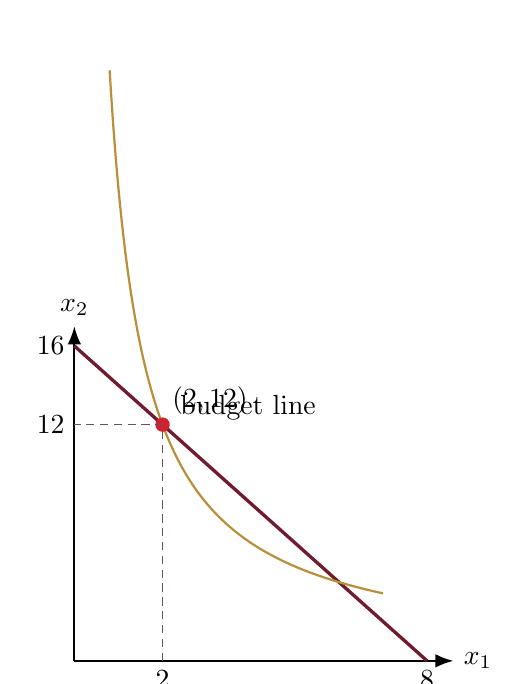
\begin{tikzpicture}[x=0.56cm,y=0.25cm,>=Latex]
  \draw[->,thick] (0,0) -- (8.6,0) node[right] {\(x_1\)};
  \draw[->,thick] (0,0) -- (0,17.0) node[above] {\(x_2\)};
  \draw[PPEBurgundy,very thick] (0,16) -- (8,0)
    node[pos=0.27,above right,black] {budget line};
  \draw[PPEGold,thick,domain=0.8:7.0,samples=90,smooth]
    plot (\x,{24/\x});
  \filldraw[PPENavarraRed] (2,12) circle (2.4pt)
    node[above right,black] {\((2,12)\)};
  \draw[densely dashed,PPEMuted] (2,0) -- (2,12) -- (0,12);
  \node[below] at (2,0) {\(2\)};
  \node[left] at (0,12) {\(12\)};
  \node[left] at (0,16) {\(16\)};
  \node[below] at (8,0) {\(8\)};
\end{tikzpicture}
\end{center}

\section{Cost minimisation and cost curves \hfill (8 points)}

\textbf{35.a Cost-minimising inputs.} For \(q=\sqrt{LK}\),
\[
MPL=\frac12\sqrt{\frac{K}{L}},
\qquad
MPK=\frac12\sqrt{\frac{L}{K}},
\qquad
\MRTS_{L,K}=\frac{MPL}{MPK}=\frac{K}{L}.
\]
Cost minimisation requires
\[
\frac{K}{L}=\frac{w}{r}=\frac41=4
\quad\Longrightarrow\quad
K=4L.
\]
The output requirement gives
\[
\sqrt{L(4L)}=2L=12
\quad\Longrightarrow\quad
\boxed{L^*=6,\qquad K^*=24.}
\]
Minimum cost is
\[
\boxed{C^*=4(6)+1(24)=48.}
\]

\textbf{35.b Cost curves and output.} From
\[
TC(q)=36+6q+q^2,
\]
we obtain
\[
\boxed{FC=36,\qquad VC(q)=6q+q^2,\qquad MC(q)=6+2q,}
\]
\[
\boxed{AFC(q)=\frac{36}{q},\qquad AVC(q)=6+q,\qquad
ATC(q)=\frac{36}{q}+6+q.}
\]
A competitive firm sets \(p=MC\), as long as \(p\geq AVC\):
\[
30=6+2q
\quad\Longrightarrow\quad
\boxed{q^*=12.}
\]
At this output,
\[
ATC(12)=\frac{36}{12}+6+12=\boxed{21}.
\]
Revenue is \(TR=30(12)=360\), while
\[
TC(12)=36+6(12)+12^2=252.
\]
Therefore
\[
\boxed{\pi=360-252=108.}
\]
The firm operates in the short run because \(p=30>AVC(12)=18\).

\section{Production technology and MRTS \hfill (7 points)}

For
\[
q=4L^{1/2}K^{1/2},
\]
\[
MPL=\frac{\partial q}{\partial L}
=\boxed{2\sqrt{\frac{K}{L}}},
\qquad
MPK=\frac{\partial q}{\partial K}
=\boxed{2\sqrt{\frac{L}{K}}},
\]
and
\[
\MRTS_{L,K}=\frac{MPL}{MPK}
=\boxed{\frac{K}{L}}.
\]

At \((L,K)=(4,9)\),
\[
q=4\sqrt{4\cdot9}=\boxed{24},
\]
\[
MPL=2\sqrt{\frac94}=\boxed{3},
\qquad
MPK=2\sqrt{\frac49}=\boxed{\frac43},
\qquad
\MRTS_{L,K}=\boxed{\frac94}.
\]

Finally,
\[
f(2L,2K)=4\sqrt{(2L)(2K)}
=2\bigl[4\sqrt{LK}\bigr]
=2f(L,K).
\]
Therefore, the production function has
\[
\boxed{\text{constant returns to scale}.}
\]

\section{Elasticity, revenue, and the Laffer curve \hfill (10 points)}

\textbf{37.a Price elasticity.} With
\[
Q=120-2P,
\qquad
\frac{dQ}{dP}=-2.
\]
At \(P=\text{\euro}20\),
\[
Q=120-2(20)=80,
\]
so
\[
\varepsilon_{Q,P}
=(-2)\frac{20}{80}
=\boxed{-\frac12}.
\]
Demand is inelastic. A small price increase therefore
\[
\boxed{\text{increases total revenue}.}
\]

\textbf{37.b Laffer curve.} Revenue is
\[
R(t)=t(40-2t)
=\boxed{40t-2t^2}.
\]
Its derivative is
\[
R'(t)=40-4t.
\]
Hence
\[
40-4t=0
\quad\Longrightarrow\quad
\boxed{t^*=10.}
\]
The negative second derivative, \(R''(t)=-4<0\), confirms a maximum. At
this tax,
\[
Q(t^*)=40-2(10)=\boxed{20},
\qquad
R(t^*)=10(20)=\boxed{200}.
\]

\begin{center}
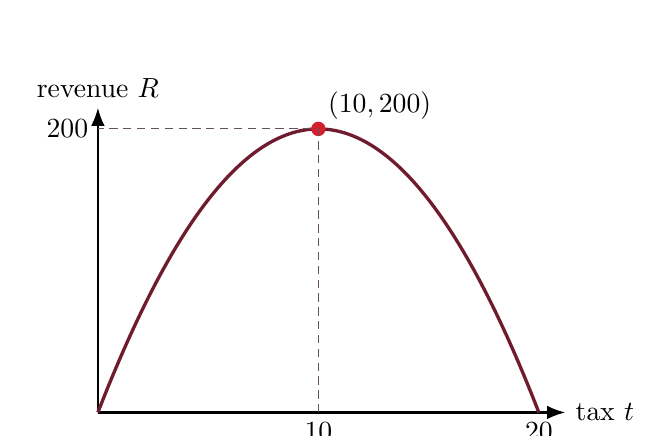
\begin{tikzpicture}[x=0.28cm,y=0.018cm,>=Latex]
  \draw[->,thick] (0,0) -- (21.2,0) node[right] {tax \(t\)};
  \draw[->,thick] (0,0) -- (0,215) node[above] {revenue \(R\)};
  \draw[PPEBurgundy,very thick,domain=0:20,samples=100,smooth]
    plot (\x,{40*\x-2*\x*\x});
  \filldraw[PPENavarraRed] (10,200) circle (2.4pt)
    node[above right,black] {\((10,200)\)};
  \draw[densely dashed,PPEMuted] (10,0) -- (10,200) -- (0,200);
  \node[below] at (10,0) {\(10\)};
  \node[left] at (0,200) {\(200\)};
  \node[below] at (20,0) {\(20\)};
\end{tikzpicture}
\end{center}

\section{Game theory \hfill (10 points)}

\begin{tipbox}
\textbf{Marking allocation.} Award 2 points for each of the five games
(\(5\times2=10\)).
\end{tipbox}

\textbf{38.a Prisoner's Dilemma.} For each player, Defect gives a higher
payoff whether the other player cooperates or defects. Thus Defect is a
strictly dominant strategy for both players, and
\[
\boxed{(\text{Defect},\text{Defect})}
\]
is the unique Nash equilibrium, with payoffs \((1,1)\). The
Pareto-superior outcome is
\[
\boxed{(\text{Cooperate},\text{Cooperate})},
\]
where both receive 3. It is not a Nash equilibrium because each player has an
incentive to deviate unilaterally and defect.

\textbf{38.b Stag Hunt.} The two pure-strategy Nash equilibria are
\[
\boxed{(\text{Stag},\text{Stag})\quad\text{and}\quad
(\text{Hare},\text{Hare}).}
\]
The payoff-dominant equilibrium is \((\text{Stag},\text{Stag})\), where both
players receive 4 rather than 3.

\textbf{38.c Dominated strategies.} For player A, Centre strictly dominates
Up and Down. For player B, Left strictly dominates Centre and Right. Hence the
unique pure-strategy Nash equilibrium is
\[
\boxed{(\text{Centre},\text{Left})}
\]
with payoffs \((5,4)\).

\textbf{38.d Non-symmetric \(3\times3\) game.} The three pure-strategy Nash
equilibria are
\[
\boxed{(\text{A},\text{Left}),\qquad
(\text{B},\text{Middle}),\qquad
(\text{C},\text{Right}).}
\]
Their respective payoffs are \((6,5)\), \((5,6)\), and \((4,4)\).

\textbf{38.e Extensive-form game.} At Player 2's decision node,
Accommodate yields 2 whereas Fight yields 0, so Player 2 chooses Accommodate.
Player 1 then compares Enter, which leads to 4, with Stay out, which yields 2.
Thus the unique SPNE is
\[
\boxed{(\text{Enter};\ \text{Accommodate after Enter}),}
\]
and the equilibrium outcome is \((4,2)\).

\section{Fill in the text \hfill (4 points)}

\begin{enumerate}[label=\textbf{\alph*.}]
  \item \(\boxed{\text{intuitive}}\) (fast and automatic is also acceptable).
  \item \(\boxed{\text{availability heuristic}}\).
  \item \(\boxed{\text{second-highest bid}}\).
  \item \(\boxed{\text{their own bid}}\).
\end{enumerate}

\section{Oligopoly and Cournot competition \hfill (8 points)}

\textbf{(i) Profit and reaction functions.} Let
\(Q_{-i}=\sum_{j\ne i}q_j\) denote the total output of firms other than
\(i\). Firm \(i\)'s profit is
\[
\begin{aligned}
\pi_i(q_i,Q_{-i})
  &= (80-q_i-Q_{-i})q_i-(20+20q_i)\\
  &= (60-q_i-Q_{-i})q_i-20.
\end{aligned}
\]
The first-order condition is
\[
\frac{\partial\pi_i}{\partial q_i}=60-2q_i-Q_{-i}=0.
\]
Thus firm \(i\)'s reaction function is
\[
\boxed{q_i=30-\frac{Q_{-i}}{2}.}
\]
\textbf{(ii) Cournot--Nash equilibrium.} In a symmetric equilibrium, every
firm supplies \(q_i=q\), so \(Q_{-i}=(N-1)q\). Hence
\[
q=30-\frac{(N-1)q}{2}
\quad\Longrightarrow\quad
\boxed{q_i^*=\frac{60}{N+1}\quad\text{for every }i.}
\]
Consequently,
\[
\boxed{Q^*=\frac{60N}{N+1},\qquad
p^*=80-Q^*=20+\frac{60}{N+1}.}
\]
Each firm's profit is
\[
\pi_i^*=(p^*-20)q_i^*-20
=\boxed{\frac{3600}{(N+1)^2}-20}.
\]

\textbf{(iii) Comparison with monopoly and perfect competition.} A monopoly
chooses \(Q\) to maximise
\[
\pi(Q)=(80-Q)Q-(20+20Q)=60Q-Q^2-20.
\]
Therefore, \(60-2Q=0\), giving
\[
\boxed{Q_M=30,\qquad p_M=50.}
\]
Under perfect competition, price equals marginal cost, so
\[
80-Q=20
\quad\Longrightarrow\quad
\boxed{Q_{PC}=60,\qquad p_{PC}=20.}
\]
For every finite \(N>1\), Cournot output and price lie between the monopoly
and competitive outcomes:
\[
\boxed{30=Q_M<Q_N^*<Q_{PC}=60,\qquad
50=p_M>p_N^*>p_{PC}=20.}
\]
As \(N\to\infty\), \(Q_N^*\to60\) and \(p_N^*\to20\). The fixed cost
does not affect the Cournot output rule because it is independent of output;
it does affect profits and any separate decision about entry.

\section{Definitions \hfill (10 points)}

\begin{description}[style=nextline,font=\sffamily\bfseries,leftmargin=3.65cm]
  \item[Pareto efficiency]
  An allocation where no person can be made better off without making at least
  one other person worse off.

  \item[Negative externality]
  An uncompensated cost imposed on a third party by a production or consumption
  decision.

  \item[Adverse selection]
  A problem caused by hidden information before a contract or transaction,
  often because one party knows more about relevant quality or risk.

  \item[Moral hazard]
  A problem caused by hidden actions after a contract, when insurance or a
  similar arrangement changes incentives.

  \item[Dominant strategy]
  A strategy that gives a player at least as high a payoff as every alternative
  for every possible action of the other players, and a higher payoff in at
  least one case (strictly dominant if higher in every case).

  \item[Nash equilibrium]
  A strategy profile in which no player can improve their payoff by changing
  their own strategy unilaterally.

  \item[Subgame-perfect Nash equilibrium]
  A Nash equilibrium that specifies a Nash equilibrium in every subgame,
  ruling out non-credible threats.

  \item[Mechanism design]
  The design of rules and incentives so that self-interested choices lead to a
  desired social or institutional outcome.

  \item[First-price auction]
  A sealed-bid auction in which the highest bidder wins and pays the amount of
  their own bid.

  \item[Present bias]
  The tendency to give disproportionately high weight to immediate rewards
  relative to future rewards.
\end{description}

\end{document}

